\section{Lineage-based Reuse}
\label{sec:reuse}

The lineage of an intermediate carries all information to identify and recompute this intermediate. LIMA leverages this characteristic in a lineage-based reuse cache for eliminating fine-grained redundancy (see Section~\ref{sec:redundancy}). Figure~\ref{fig:reuse} gives an overview of our reuse approach. In this section, we describe (1) the lineage cache organization, and multi-level reuse of intermediates for functions, blocks, and operations, (2) partial reuse of operations with compensations, (3) cost-based eviction policies, (4) compiler-assisted reuse (e.g., rewrites), and (5) remaining limitations and future work.

\subsection{Multi-Level Full Reuse}
\label{subsec:mlreuse}

As the foundation of lineage-based reuse, we establish a cache that maps lineage traces to cached, in-memory data objects. Here, we describe a holistic design for a robust system integration.

\textbf{Lineage Cache:} The basic architecture of the lineage cache---as shown in Figure~\ref{fig:reuse}---comprises a hash map from lineage items (i.e., lineage traces of values) to cached values. These values can be matrices, frames, or scalars and are wrapped into lineage cache entries that hold additional metadata such as the data type, cache status, computation time, access timestamps, and eviction scores. The cache size is a configurable fraction of the maximum heap size (5\% by default). Other configurations include the set of reusable instruction opcodes, the used eviction policy, and related parameters.

\textbf{Full Reuse:} During runtime, we then trace lineage \emph{before} instruction execution, and use the obtained lineage item to probe the lineage cache for existing outputs. Full reuse refers to an operation-level reuse of a previously computed output in full, that is, without any compensations. If this probe succeeds, we obtain the cached value, put this value into the symbol table of live variables, and skip the instruction. If the value does not yet exist in the cache, we execute the instruction and additionally store its output(s) in the lineage cache. The probing leverages the \emph{compare} functionality (via \texttt{hashCode()} and \texttt{equals()}) as described in Section~\ref{sec:tracing}. The time complexity of na\"ive \texttt{hashCode} and \texttt{equals} implementations are linear in the size of the lineage trace. However, due to materialized hash codes, we get constant complexity for constructing and hashing a new lineage item over existing lineage inputs, and using the hash codes for pruning\footnote{Long lineage traces with repeated structure are prone to hash collisions due to integer overflows. We handle such overflows with separate hash functions.}---in \texttt{equals} calls---works very well in practice. The reuse logic is integrated in the main instruction execution code path, which seamlessly applies to all instructions. In addition, making the set of cacheable instructions and data types configurable also avoids unnecessary cache pollution, and ensures correctness (e.g., for update-in-place indexing). 

\begin{figure}[!t]
	\centering
	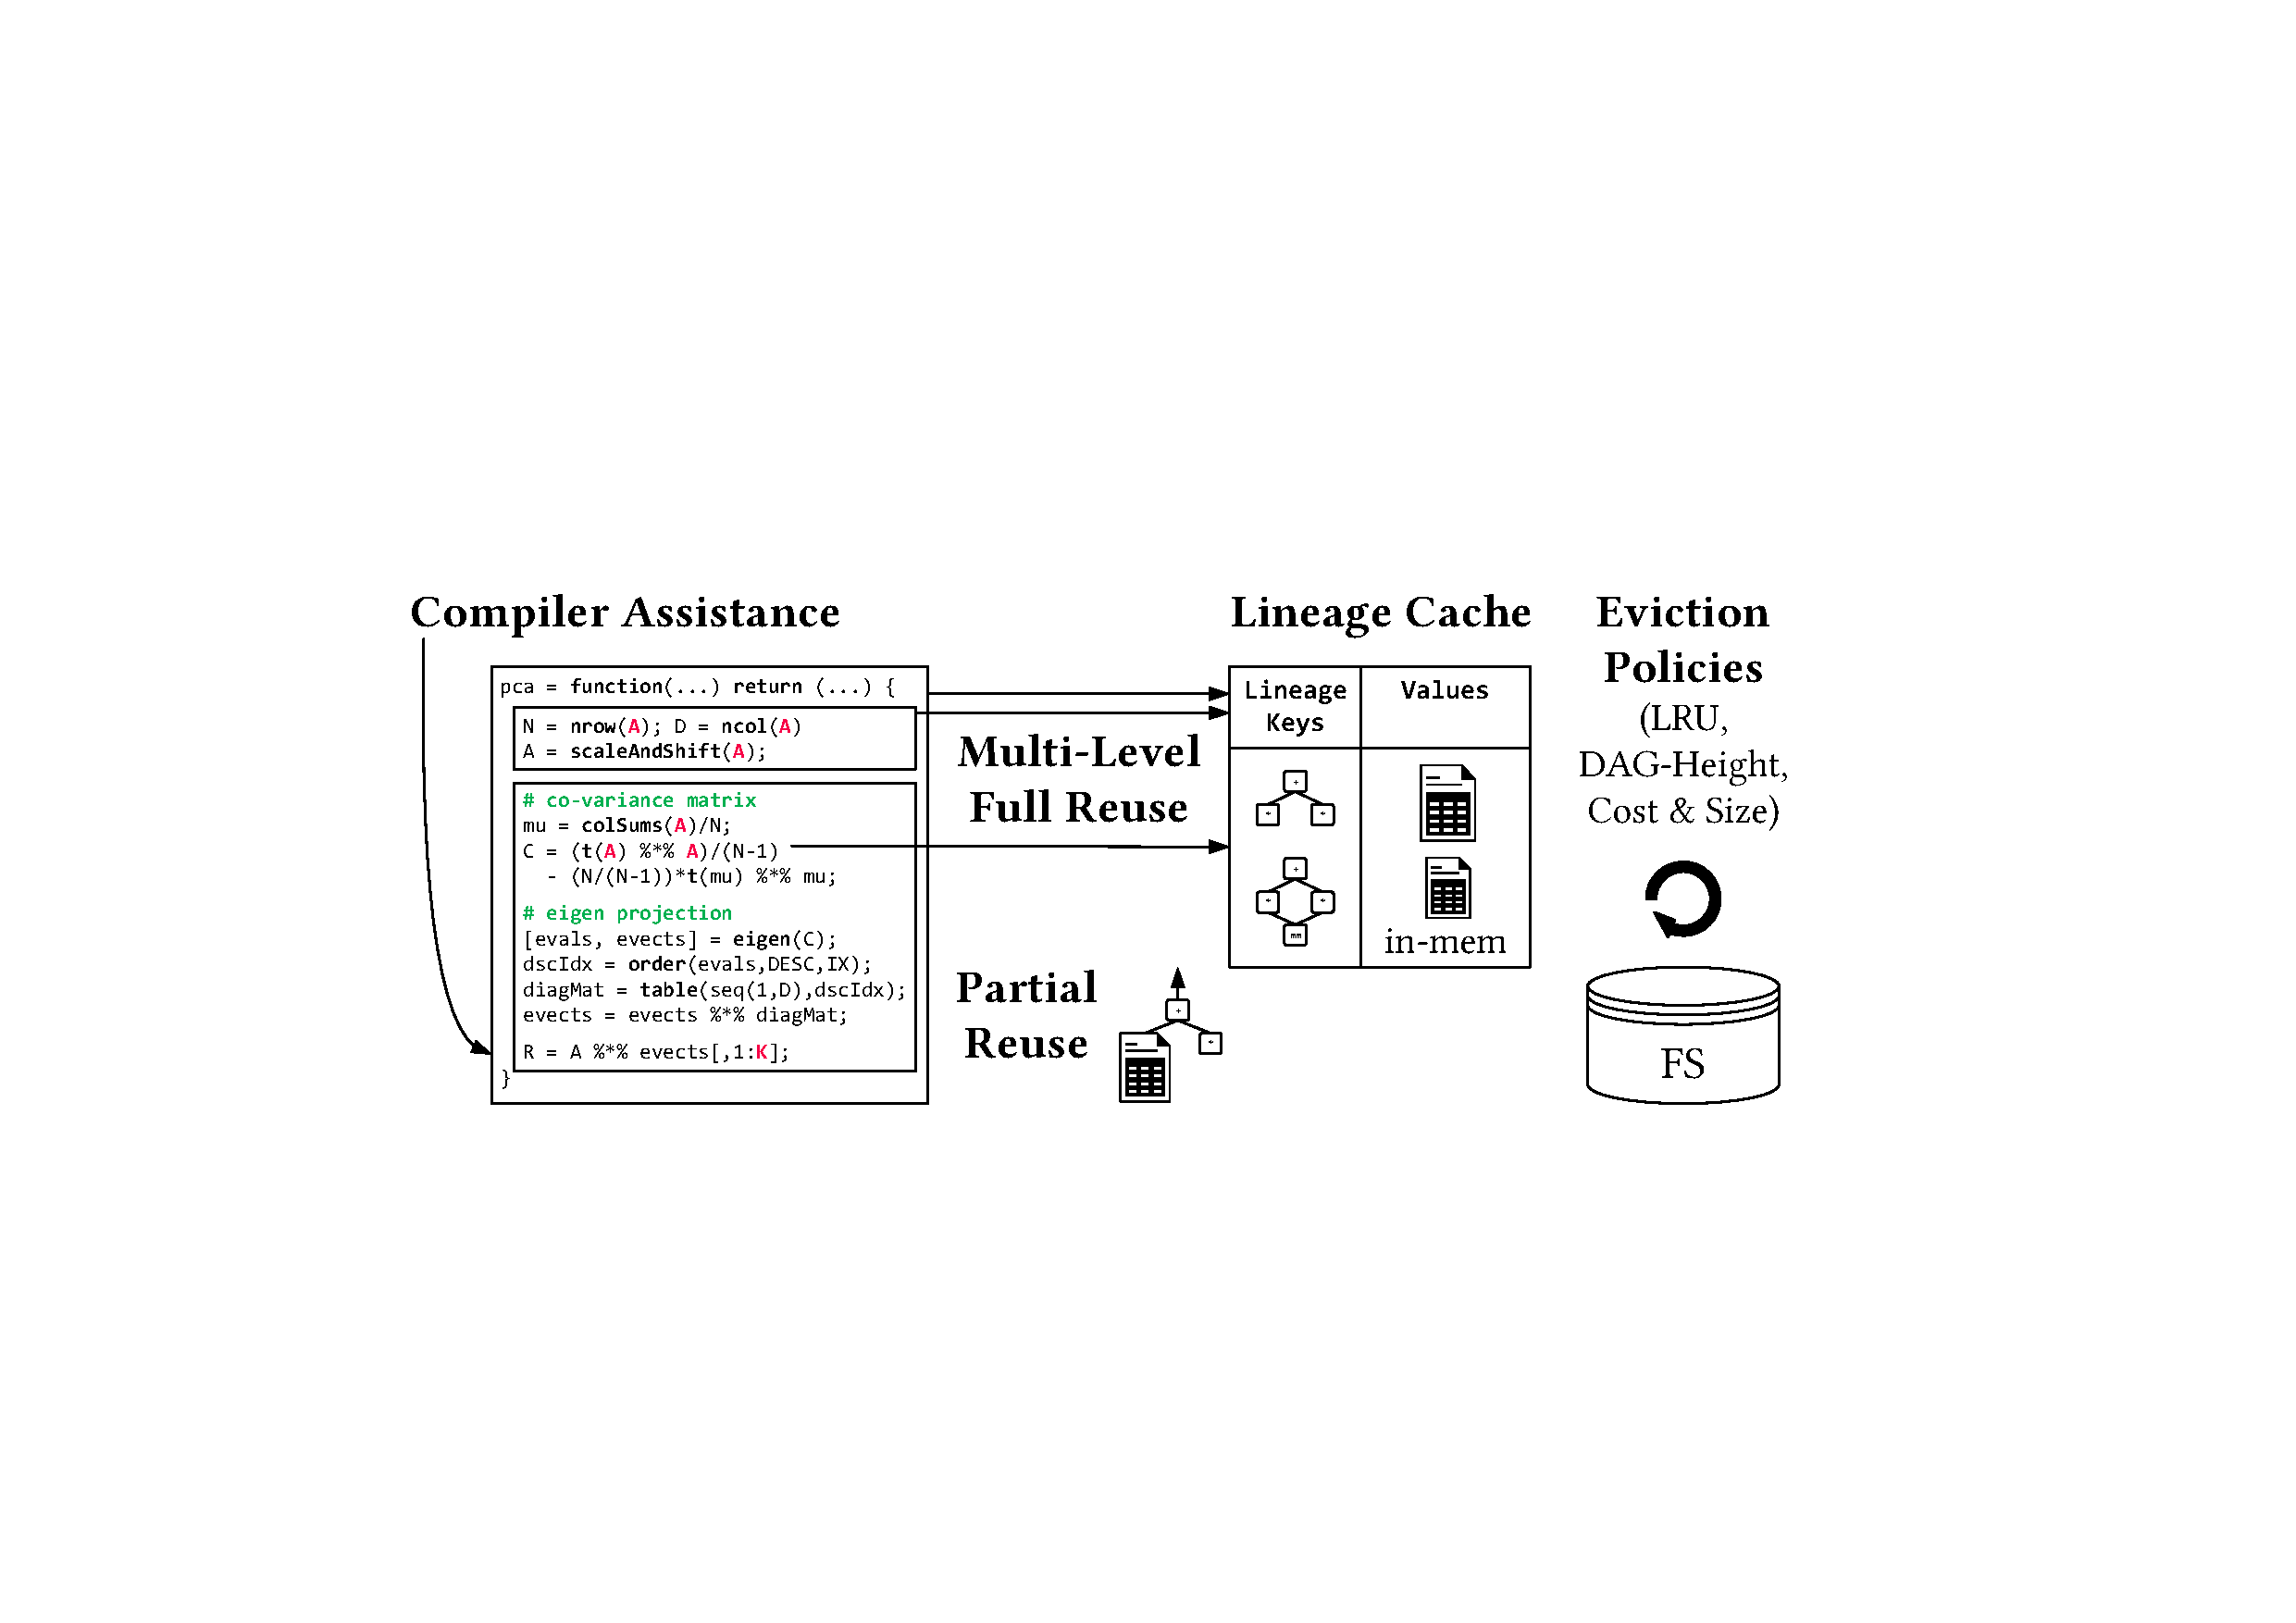
\includegraphics[scale=0.32]{figures/reuse}
	\vspace{-0.25cm}
	\caption{\label{fig:reuse}Overview Lineage-based Reuse.}
\end{figure}

\textbf{Multi-level Reuse:} Our basic full reuse eliminates fine-grained redundancy at operation level in a robust manner. However, this approach is suboptimal for coarse-grained redundancy (e.g., reuse of entire functions) because it still requires a pass over all instructions and reuse of their  cached outputs. Inspired by recent work on alternative probing strategies in CO~\cite{DerakhshanMARM20} and pruning in HELIX~\cite{XinMMLSP18}, we augment the basic reuse by a multi-level reuse approach to avoid cache pollution and interpretation overhead. Our basic idea is to leverage the hierarchical program structure of functions and control flow blocks (see background in Section~\ref{sec:mlsys}) as natural probing and reuse points. As pre-processing step, we determine and materialize if a given function or block is deterministic, i.e., does not include any non-deterministic operations or function calls. A block is similar to a function as it has specific inputs and outputs, which we obtain from live variable analysis. During runtime, we then construct a special lineage item that represents the function inputs, function call, and bundles all function outputs. If a deterministic function is called with the same inputs, we can thus, directly reuse its outputs; otherwise we execute the function and also bind cached outputs to the special lineage item. Multi-level reuse is orthogonal to lineage deduplication, but internally leverages shared infrastructure.

\begin{example}[PCA Multi-level Reuse] Figure~\ref{fig:reuse} also illustrates this concept of multi-level reuse, where we first probe the entire \texttt{pca} (principal component analysis) function call. If we cannot reuse, we probe individual blocks (e.g., the block around \texttt{scaleAndShift}), and finally, individual operations (e.g., $\mat{A}^{\top}\mat{A}$ as used in \texttt{pca} and \texttt{lmDS}).
\end{example}

\textbf{Task-parallel Loops:} Similar to lineage tracing, supporting task-parallelism requires further lineage cache extensions. First, multi-threaded \texttt{parfor} workers concurrently probe and update the shared lineage cache. This concurrency requires a thread-safe lineage cache, which we ensure via latches and a careful implementation that keeps the critical sections small and prevents deadlocks. Second, we use lineage cache ``placeholders'' (empty lineage cache entries) to avoid redundant computation in parallel tasks. For example, consider the following hyper-parameter tuning loop:
\begin{lstlisting}
 1: parfor(i in 1:nrow(lambda))
 2:   B[,i] = lmDS(X=X, y=Y, reg=lambda[i,1]);
\end{lstlisting}
For instance, k=32 iterations might run in parallel here, and during the first wave of iterations $\mat{X}^{\top}\mat{X}$ and $\mat{X}^{\top}\mat{y}$ are not yet available for reuse. This redundancy matters because we should rather spend the parallelism in individual operations if needed. Hence, the first thread puts a placeholder in the cache. Other threads then find this placeholder and block on obtaining its matrix, frame, or scalar until the first thread adds the computed value back to the placeholder.


\subsection{Partial Operation Reuse}
\label{sec:partial}

Beyond multi-level full reuse, LIMA also eliminates \emph{partial operation redundancy} via partial reuse. Partial reuse refers to an operation-level reuse of a previously computed output, augmented by a compensation plan of reused or computed operations. 

%TODO only if large enough

\textbf{Partial Reuse:} If full reuse is not possible, we quickly probe different partial reuse opportunities, and only if none applies, fallback to normal instruction execution. This probing for partial reuse evaluates an ordered list of rewrites of source-target patterns. If the current lineage item (before execution) matches a source pattern, and components of the target pattern are available in the lineage cache, we construct a \emph{compensation plan} to compute the result. Similar to constant folding, we put reusable intermediates of the target pattern into a temporary symbol table, construct an operation DAG for the remaining operations, and then, compile and execute actual runtime instructions to obtain the results. The rewrites are hand-written and can include cost-based constraints. Our existing rewrites focus primarily on real use cases and patterns with \texttt{rbind}, \texttt{cbind}, and indexing in combination with matrix multiplications, column or row aggregates, and element-wise operations.

\textbf{Example Rewrites:} Our set of partial rewrites comprises 14 meta rewrites with internal variants. Below equation shows selected examples, where $\mat{X}\,\mat{Y}$ is a matrix multiply, $\odot$ and $+$ are element-wise multiply and addition, and $\textbf{dsyrk}(\mat{X})$ is a shorthand for $\mat{X}^{\top}\mat{X}$.
\[\begin{split}
\textbf{rbind}(\mat{X},\Delta\mat{X})\,\mat{Y} &\rightarrow \textbf{rbind}(\mat{X}\,\mat{Y}, \Delta\mat{X}\,\mat{Y})\\
\mat{X}\,\textbf{cbind}(\mat{Y},\Delta\mat{Y}) &\rightarrow \textbf{cbind}(\mat{X}\,\mat{Y}, \mat{X}\,\Delta\mat{Y})\\
\mat{X}\,\textbf{cbind}(\mat{Y},\mat{1}) &\rightarrow \textbf{cbind}(\mat{X}\,\mat{Y}, \textbf{rowSums}(\mat{X}))\\
\mat{X}\,(\mat{Y}[,1{\,:\,}k]) &\rightarrow (\mat{X}\,\mat{Y})[,1{\,:\,}k]\\
\textbf{dsyrk}(\textbf{rbind}(\mat{X},\Delta\mat{X})) & \rightarrow \textbf{dsyrk}(\mat{X}) + \textbf{dsyrk}(\Delta\mat{X})\\
\textbf{dsyrk}(\textbf{cbind}(\mat{X},\Delta\mat{X})) & \rightarrow \textbf{rbind}(
	\textbf{cbind}(\textbf{dsyrk}(\mat{X}), \mat{X}^{\top}\Delta\mat{X}),\\
	 &\qquad\quad\textbf{cbind}(\Delta\mat{X}^{\top}\,\mat{X}, \textbf{dsyrk}(\Delta \mat{X})))\\
\textbf{cbind}(\mat{X},\Delta\mat{X}) \odot \textbf{cbind}(\mat{Y},\Delta\mat{Y}) &\rightarrow \textbf{cbind}(\mat{X}\odot\mat{Y},\Delta\mat{X}\odot\Delta\mat{Y})\\
\textbf{colAgg}(\textbf{cbind}(\mat{X}, \Delta\mat{X})) &\rightarrow \textbf{cbind}(\textbf{colAgg}(\mat{X}), \textbf{colAgg}(\Delta\mat{X}))\\
\end{split}\]
Similar rewrites have been used for incremental linear algebra programs \cite{NikolicEK14}, linear algebra simplification rewrites \cite{BoehmBERRSTT14,ElgamalLBETRS17,WangHSHL20,FangSW020,JiaPTWZA19}, and hand-optimized cross validation primitives \cite{KunftKSBRM19}. In contrast, we apply them during lineage-based reuse or recompilation. Application examples are \texttt{lm} and \texttt{scaleAndShift} with and without intercept, cross validation, as well as \texttt{stepLm} \cite{VenablesR02,BoehmADGIKLPR20}, a feature selection algorithm that repeatedly appends additional features.

\subsection{Cache Eviction}
\label{sec:eviction}

Lineage cache eviction ensures that the size of cached objects does not exceed the configured budget. Important aspects are the cache management, and dedicated cost-based eviction policies.

\textbf{Cache Management:} Given an absolute memory budget $B$ (by default, 5\% of heap size), intermediates of size smaller than $B$ are subject to caching. On adding such an object $o$ to the cache, we get its in-memory size $s(o)$ and trigger eviction if the cache size $S + s(o)$ exceeds $B$. Objects under eviction management (excluding empty placeholders), are then added to a priority queue $\mat{Q}$ that orders objects for eviction according to eviction-policy-specific scoring functions. An active eviction then pulls and evicts items in order until the budget constraint $S \leq B$ is met. The eviction of an object is either by deletion or by spilling to disk, where we only spill objects whose re-computation time exceed the estimated I/O time. We perform additional bookkeeping to allow identifying such spilled cache entries. With multi-level reuse, multiple cache entries might refer to the same object but exhibit different costs (e.g., function versus operation). In such scenarios, we defer the spilling of an entry group until all group entries are pulled for eviction.

\textbf{Statistics and Costs:} As a basis for our eviction policies and user-facing statistics, we collect various statistics. On entering the cache, we obtain (1) the measured function or operation execution time $c(o)$ of cached objects, and (2) the height $h(o)$ of related lineage traces (distance from leaves). During cache usage, we further gather (3) the last access timestamp $T_a(o)$, and (4) the number of references (\#hits $r_h$, \#misses $r_m$). Additionally, we estimate (5) the spill (write) and restore (read) times of cached objects. We obtain the sizes in memory $s_m(o)$ and on disk $s_d(o)$ from the data characteristics, and scale $s_d(o)$ with expected read/write bandwidths for dense and sparse matrices, or frames. For adaptation to the underlying hardware, we adjust these expected bandwidths (starting heuristics) as an exponential moving average with the measured I/O times.

\begin{table}[!t]
	\centering \small \setlength\tabcolsep{12pt}
	\caption{\label{tab:evict}Eviction Policies and Scoring Functions.}
	\vspace{-0.4cm}
	\begin{tabular}{cc}
	  \toprule
		\textbf{Eviction Policy} & \textbf{Eviction Scoring Function} \\
		\midrule
    \textbf{LRU}          & $\argmin_{o \in \mat{Q}} \quad T_a(o) /\theta$ \\
		\textbf{DAG-Height}   & $\argmin_{o \in \mat{Q}} \quad 1/h(o)$ \\
		\textbf{Cost \& Size} & $\argmin_{o \in \mat{Q}} \quad (r_h+r_m)\cdot c(o)/s(o)$\\
		\bottomrule
	\end{tabular}
	\normalsize
\end{table}

\textbf{Eviction Policies:} The chosen eviction policy determines the order of eviction. Table~\ref{tab:evict} shows the supported policies and their scoring functions to get the next item for eviction. First, \emph{LRU} orders by a normalized last access timestamp $T_a(o)/\theta$. Second, \emph{DAG-Height} assumes that deep lineage traces have less reuse potential, and orders accordingly by $1/h(o)$. Third, similar to CO's \cite{DerakhshanMARM20} artifacts-materialization logic, \emph{Cost\&Size} aims to preserve objects with high computation costs $c(o)$ to size $s(o)$ ratio, scaled by $(r_h+r_m)$ (\#accesses) to account for global reuse potential, and evicts the object with minimal $(r_h+r_m)\cdot c(o)/s(o)$. While \emph{LRU} performs good in pipelines with temporal reuse locality, \emph{DAG-Height} handles mini-batch scenarios better, where batches are sliced from the input dataset and reused across epochs. However, both \emph{LRU} and \emph{DAG-Height} make strong assumptions. In contrast, \emph{Cost\&Size}, together with disk spilling, performs well in a wide variety of scenarios as it tunes for global reuse utility (saved computation by size). Hence, \emph{Cost\&Size} is our default. We abandoned an Hybrid (weighted) strategy in favor of this parameter-free policy. Adaptive policies like ARC \cite{MegiddoM03} that balance recency and utility is interesting future work.

\subsection{Compiler Assistance}
\label{sec:compassisted}

Lineage-based reuse at runtime level is valuable because many reuse opportunities are unknown during compilation due to conditional control flow. However, a pure runtime approach is not enough because some patterns are detected too late (after part of these patterns are already evaluated). We address this dilemma by augmenting our runtime lineage cache with compiler assistance.

\textbf{Unmarking Intermediates:} In order to avoid cache pollution---and thus, unnecessary probing, and evictions---we added a program-level rewrite that unmarks intermediates for reuse. Unmarking disables probing and caching of a specific operation instance---even if its opcode is in the set of qualifying operations---if it is unlikely to be reused over the program lifetime. This rewrite has access to the entire control program and operation DAGs of a script, but performs unmarking conservatively because the lineage cache is used across script invocations through SystemDS' programmatic APIs. Examples are the computation of fully updated, local variables that depend recursively on previous loop iterations.

\textbf{Reuse-aware Rewrites:} We further added several reuse-aware DAG rewrites, which---if lineage-based reuse is enabled---prefer patterns that create additional reuse opportunities without hurting the runtime of normal plan execution (by cost estimates). There are several examples. First, for k-fold cross validation over \texttt{lm}, we construct the feature matrix from a list of folds $\mat{X} = \textbf{rbind}(\text{lfolds})$ and compute $\mat{X}^{\top}\mat{X}$ and $\mat{X}^{\top}\mat{y}$. Applying, after function inlining, the partial rewrite $\textbf{dsyrk}(\textbf{rbind}(\mat{X},\Delta\mat{X})) \rightarrow \textbf{dsyrk}(\mat{X}) + \textbf{dsyrk}(\Delta\mat{X})$ for $k-1$ folds during compilation allows us to avoid the repeated $\textbf{rbind}$ operations, and compute and reuse the matrix multiplications just once per fold. Second, consider different feature projections via $\mat{R} = \mat{A}\,(\mat{evect}[,1:K])$ in PCA from Figure~\ref{fig:reuse}. If an outer loop calls PCA for different $K$, a dedicated rewrite speculatively computes $\mat{A}\,\mat{evect}$ for more efficient partial reuse.

\textbf{Reuse-aware Recompilation:} SystemDS compiler marks a DAG for recompilation if sizes (dimensions, sparsity) of intermediates are unknown, and later adaptively recompiles plans during runtime at natural block boundaries. We extended this recompilation with further reuse-aware rewrites as it provides a great balance between reduced uncertainty of conditional control flow, and large-enough optimization scope. For example, in \texttt{stepLm} such rewrites allow partial reuse for $\textbf{dsyrk}(\textbf{cbind}(\mat{X},\Delta\mat{X}))$, but also avoid the expensive materialization of $\textbf{cbind}(\mat{X},\Delta\mat{X}))$. Internally, the rewrites from Section~\ref{sec:partial} are shared by both, partial reuse and recompilation.

\subsection{Limitations}
\label{sec:limitations}

Similar to Section~\ref{sec:limits1}, we summarize limitations, which we see as out-of-scope of the initial LIMA framework and thus, future work.
\begin{itemize}
\item \emph{Unified Memory Management:} SystemDS has multiple memory managers such as the buffer pool for live variables, operation memory, and now the lineage cache. The static partitioning can cause unnecessary evictions, which makes a unified memory manager (as in Spark \cite{UnifiedMem}) desirable.
\item \emph{Multi-level Partial Reuse:} Conceptually, we could also apply the idea of partial reuse---by composition---to blocks and functions. However, this would introduce significant complexity.
\item \emph{No Multi-location Caching:} Although we trace lineage for both local and distributed operations, the lineage cache currently only applies to local, in-memory objects. %no RDDs, broadcasts, or multiple devices
\item\emph{Materialization of Lineage Cache:} Our reuse cache is designed for process-wide sharing, which also applies to collaborative notebook environments. Reusing across processes would require extensions for speculative materialization and cleanup.
\end{itemize}

